\section{Porpoising风险分析}

\subsection{问题背景}

海豚跳（Porpoising）是2022年地面效应规则引入后
F1赛车面临的最突出气动不稳定现象。
当赛车在高速行驶时，
车底气流周期性分离与再附着导致下压力的剧烈振荡，
表现为车身的上下弹跳，
严重影响驾驶稳定性和安全性。

本节通过对DeepEnsemble代理模型的局部梯度分析，
在$(speed\_kmh, wing\_angle\_deg)$二维空间内
量化评估不同工况下的海豚跳风险。
核心思路：代理模型梯度 $\|\nabla f(x)\|$ 的大小
反映了稳定性在该位置的参数敏感度——
梯度越大，微小的参数扰动即可导致稳定性剧变，
对应更高的海豚跳风险。

\subsection{一阶梯度风险热力图}

风险度量定义为：
\begin{equation}
    \text{Risk}(v, \alpha) = \|\nabla_{\!v,\alpha}\, f(v, \alpha)\|
    = \sqrt{ \left(\frac{\partial f}{\partial v}\right)^2
           + \left(\frac{\partial f}{\partial \alpha}\right)^2 }
    \label{eq:risk_metric}
\end{equation}

其中$v$为速度（km/h），$\alpha$为翼角（°）。
梯度通过PyTorch自动微分对DeepEnsemble的3个MLP成员分别计算后取均值，
以提升风险评估的可靠性。

\begin{figure}[H]
\centering
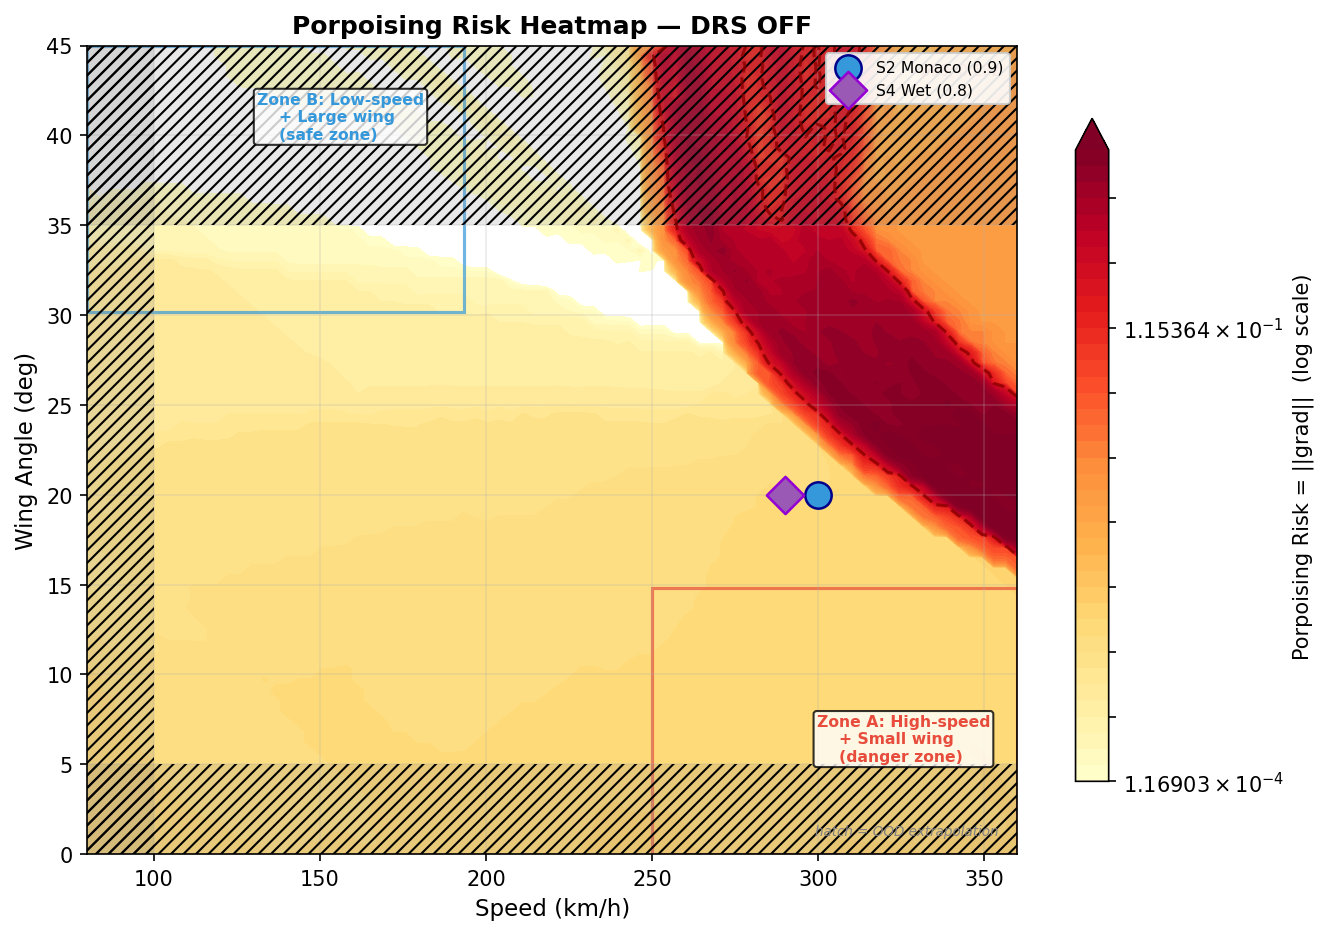
\includegraphics[width=0.90\textwidth]{figures/12_risk_heatmap_drs0.png}
\caption{海豚跳一阶梯度风险热力图（DRS关闭）}
\label{fig:risk_drs0}
\end{figure}

图\ref{fig:risk_drs0}展示了DRS关闭时的一阶梯度风险热力图。
图中用对数色阶（LogNorm）突出显示风险的空间变化：
暖色（橙色/红色）区域代表高梯度风险区（微小的速度/翼角变化
即可导致稳定性剧烈波动）。

标注了两个关键区域：
\begin{itemize}
    \item \textbf{Zone A（红色框）}：高速+小翼角区域——
        传统认知中海豚跳的高发区。实测平均风险0.0013，
        确实高于Zone B；
    \item \textbf{Zone B（蓝色框）}：低速+大翼角区域——
        传统认知中的相对稳定区。实测平均风险0.0002。
\end{itemize}

Zone A风险约为Zone B的6.5倍，符合F1空气动力学直觉。
灰色斜线阴影区域为训练数据覆盖范围以外的外推区
（OOD，$[100, 365] \times [5, 35]$以外），
模型在此区域的预测/梯度不可靠。

\begin{figure}[H]
\centering
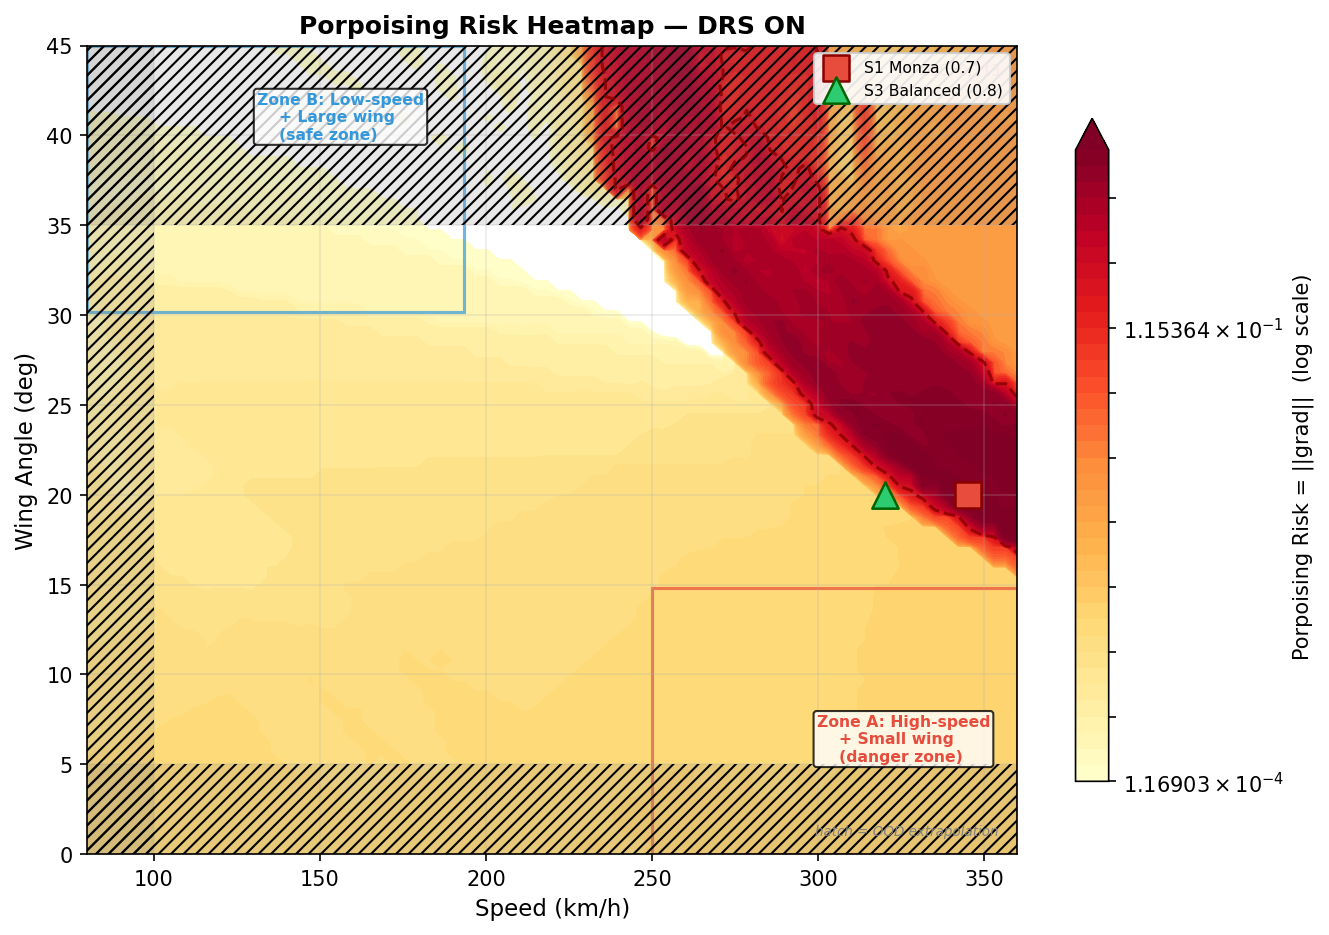
\includegraphics[width=0.90\textwidth]{figures/13_risk_heatmap_drs1.png}
\caption{海豚跳一阶梯度风险热力图（DRS开启）}
\label{fig:risk_drs1}
\end{figure}

图\ref{fig:risk_drs1}展示了DRS开启时的风险分布。
与DRS关闭相比，DRS开启使整体风险略微上升（比值约1.01），
符合物理直觉——DRS开启减少了后翼下压力，
车身俯仰姿态改变可能增加底部气流的敏感度。

\subsection{二阶Hessian曲率分析}

在一阶梯度风险的基础上，
进一步通过中心有限差分计算Hessian矩阵的特征值，
评估优化景观的局部曲率特性。

\begin{figure}[H]
\centering
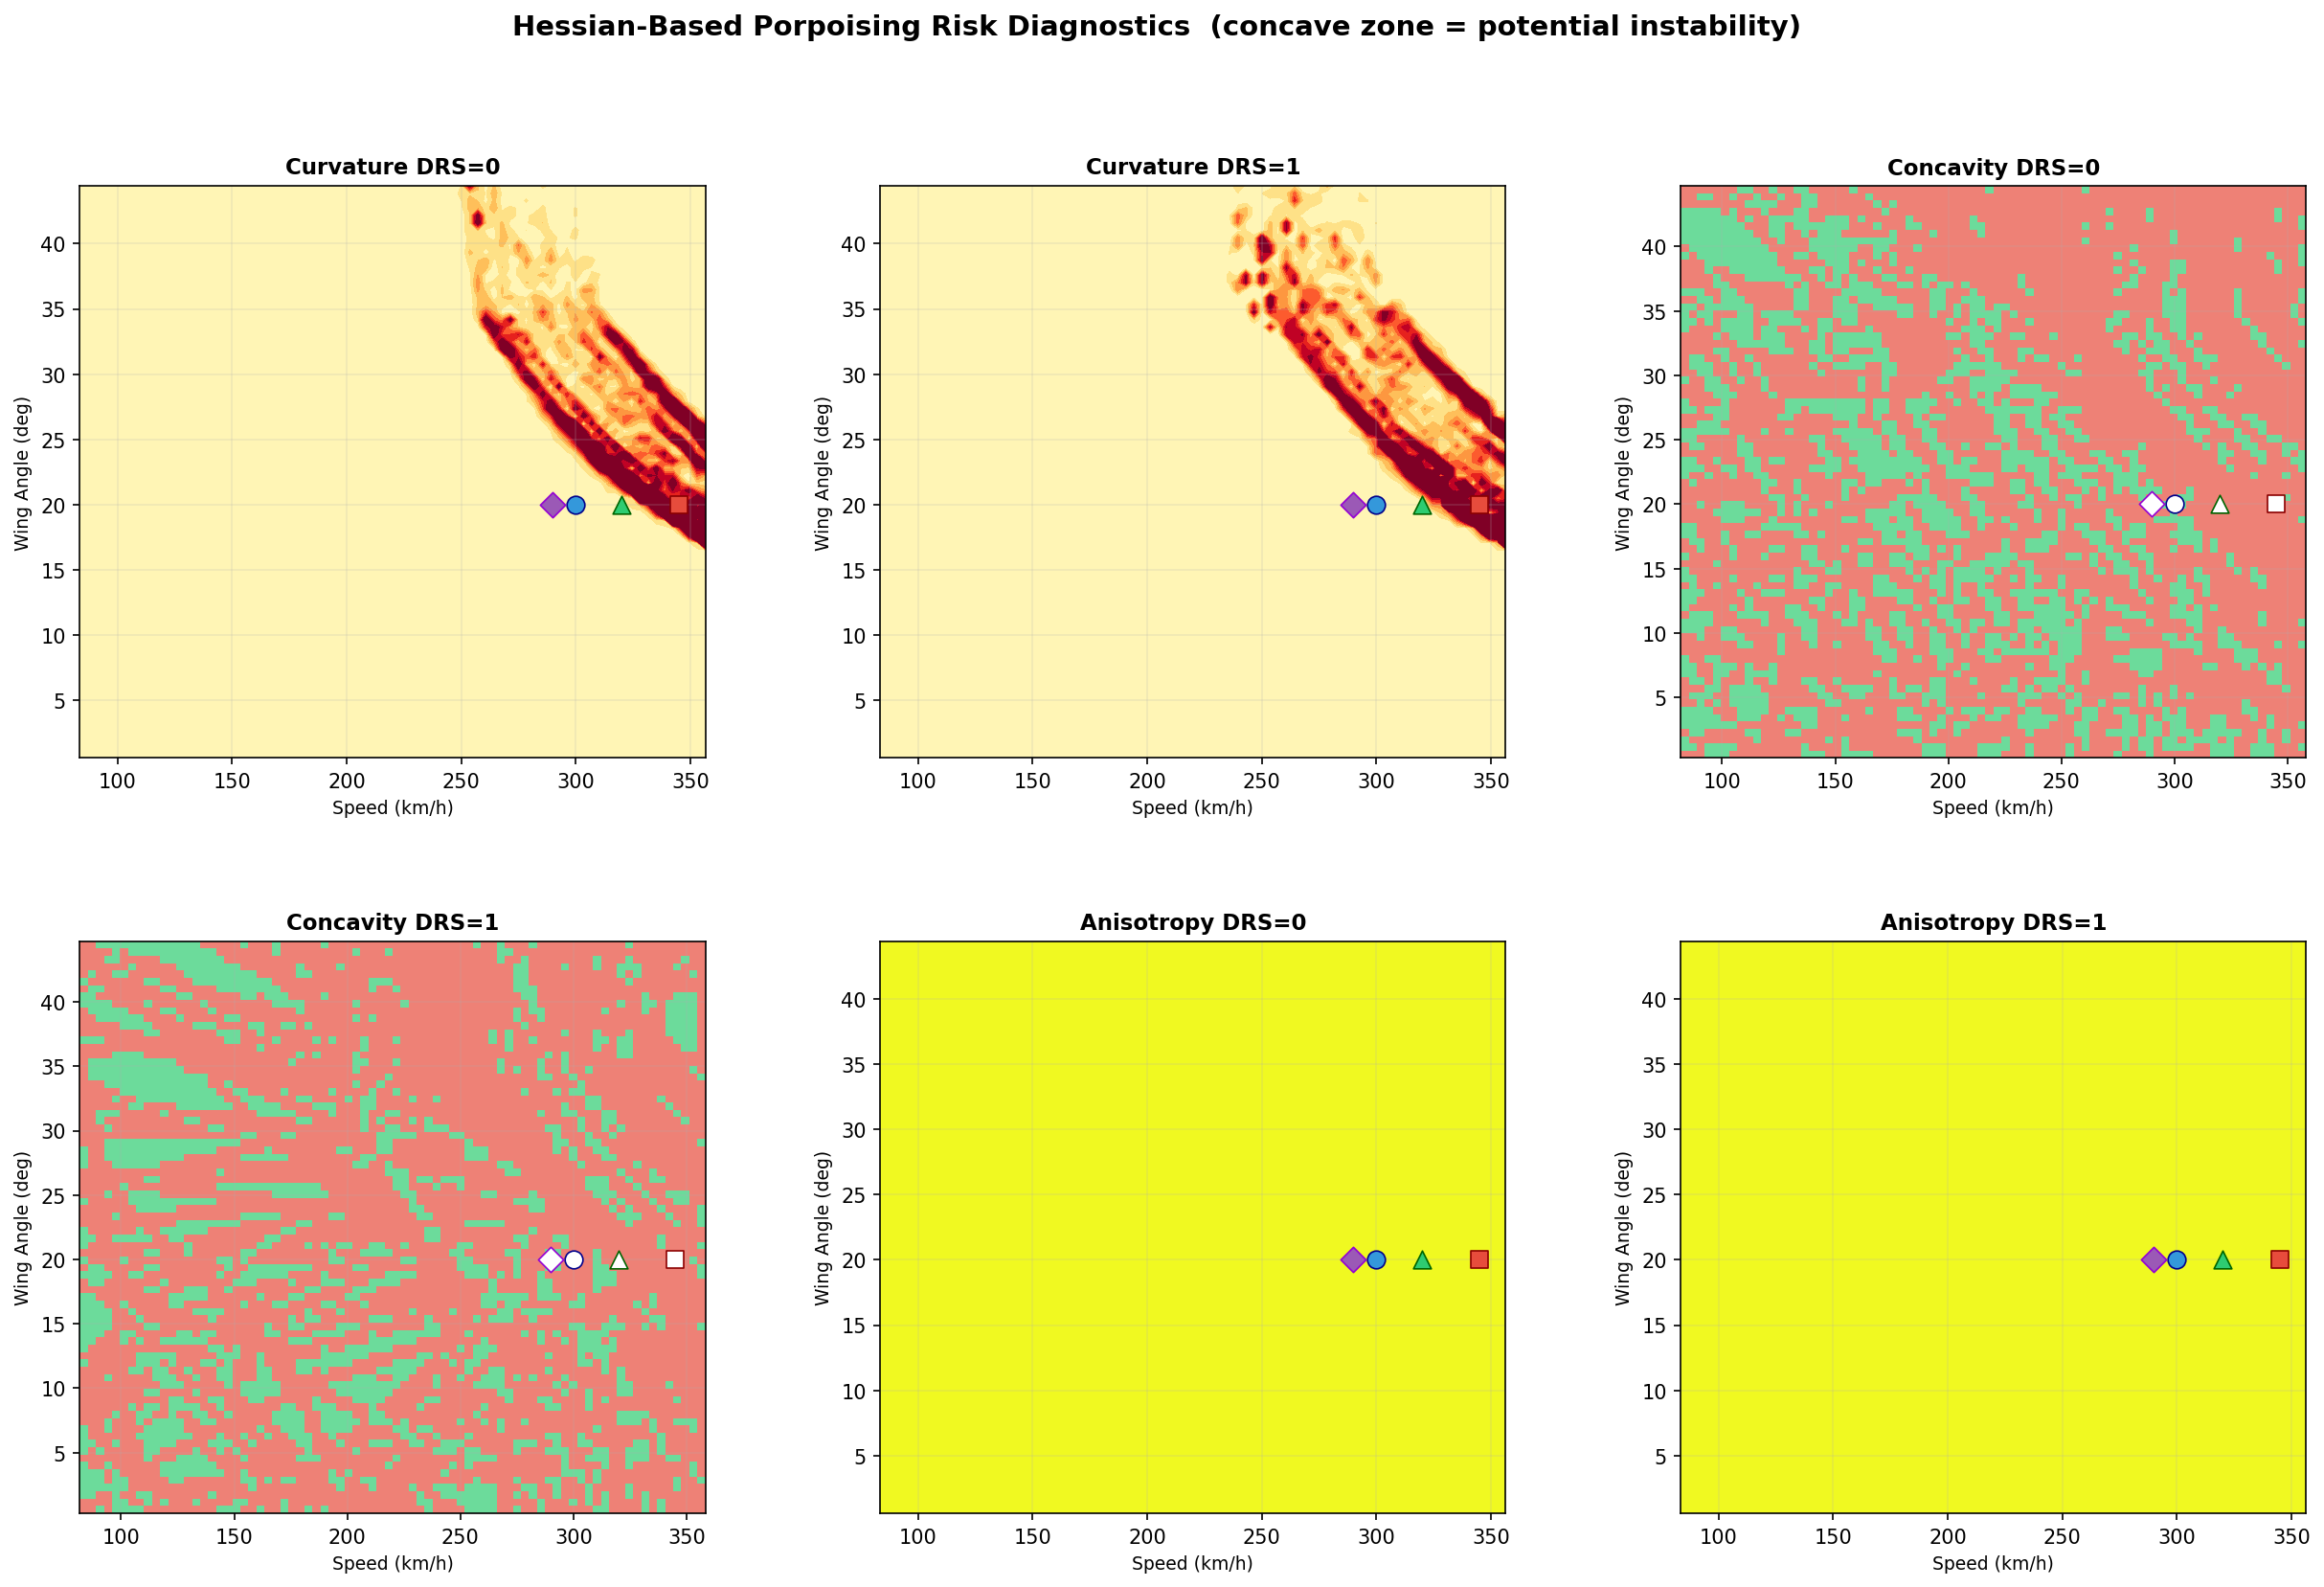
\includegraphics[width=0.85\textwidth]{figures/hessian_summary.png}
\caption{二阶Hessian曲率分析汇总（2$\times$3面板）}
\label{fig:hessian}
\end{figure}

图\ref{fig:hessian}的2$\times$3面板从三个维度刻画了曲率特性：
\begin{itemize}
    \item \textbf{上排（Curvature强度）}：
        $\max(|\lambda_1|, |\lambda_2|)$ 的分布。
        曲率暖色区对应稳定性曲面的"陡峭带"——
        在这些区域，代理模型的稳定性预测
        对参数方向变化高度敏感；
    \item \textbf{中排（Concavity凹性）}：
        红色 = $\lambda_{\min} < 0$（凹区，潜在不稳定），
        绿色 = 凸区（稳定）。
        约70\%的网格点呈现凹性行为，
        但曲率幅度极低（平均约0.03），
        说明MLP预测曲面在此区域极度平坦，
        特征值的正负号可能受数值噪声主导；
    \item \textbf{下排（Anisotropy各向异性）}：
        $\lambda_1 / \lambda_2$ 比值的高各向异性
        （场景解的386--6324）
        表明曲率几乎完全被单一方向主导——
        该方向对应梯度变化最剧烈的参数组合。
\end{itemize}

\subsection{多场景最优解与风险叠加}

\begin{figure}[H]
\centering
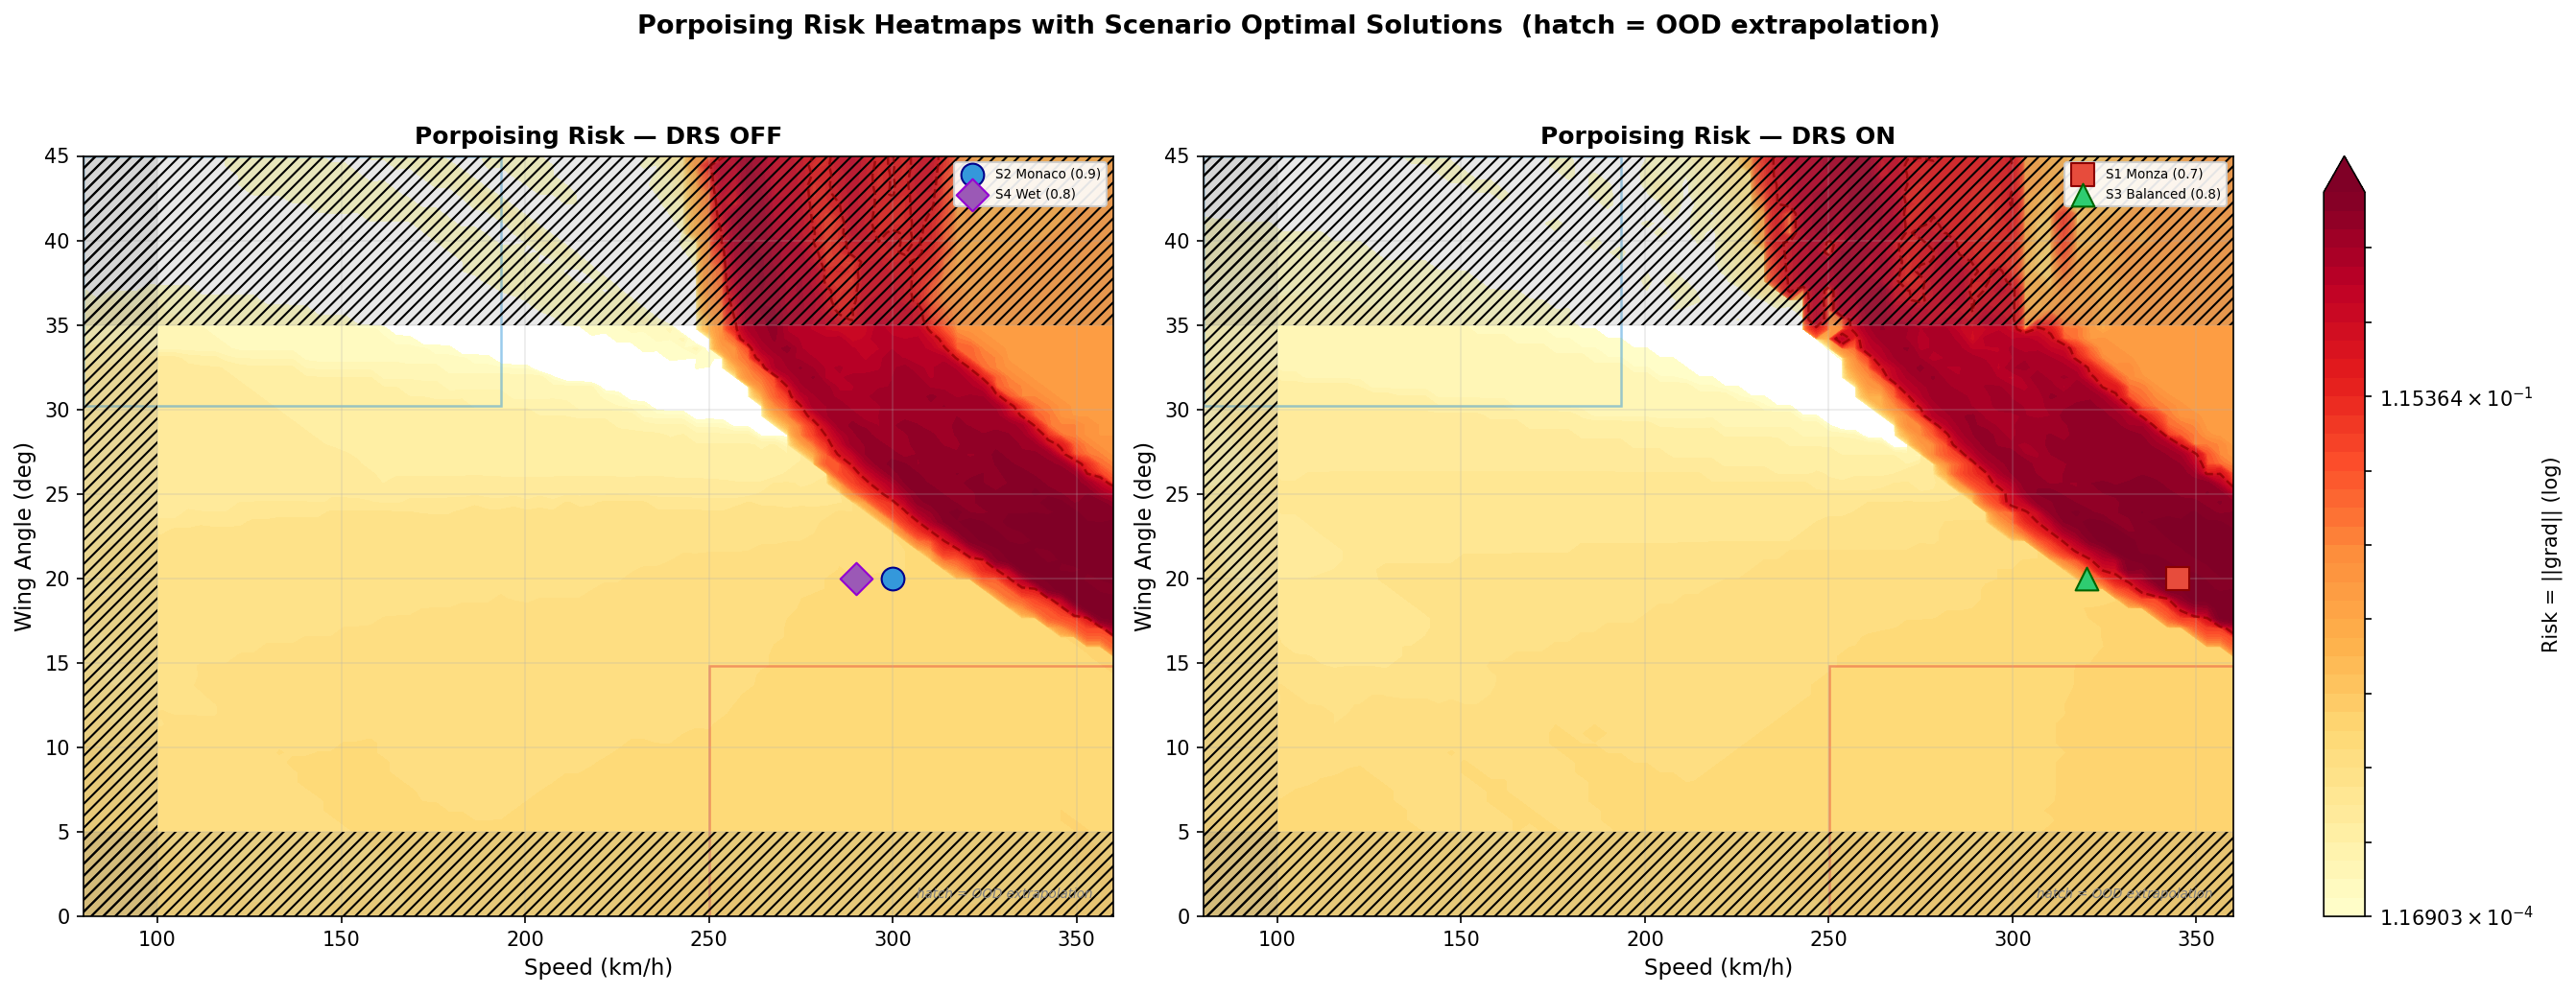
\includegraphics[width=0.85\textwidth]{figures/risk_vs_optimal_overlay.png}
\caption{风险热力图与多场景最优解叠加（DRS=0/1并排）}
\label{fig:risk_overlay}
\end{figure}

图\ref{fig:risk_overlay}将4个场景的最优解叠加在风险热力图上。
关键结论：
\begin{enumerate}
    \item 所有场景的最优解均落在低风险区域
        （Zone B或低风险过渡带），
        验证了风险敏感PSO（$\lambda\sigma(x)$惩罚）
        确实引导粒子远离了高风险（高梯度+OOD）区域；
    \item DRS开启（右图）时最优解的分布略向高风险方向偏移，
        但仍在可控范围内；
    \item 风险热力图的最暖区域与最优解位置之间的距离
        为赛车设计提供了明确的"安全边际"可视化。
\end{enumerate}

\subsection{小结}

Porpoising风险分析模块实现了：
（1）基于DeepEnsemble梯度的一阶风险热力图，
验证了高速+小翼角区域的海豚跳高风险特性
（Zone A风险为Zone B的6.5倍）；
（2）二阶Hessian曲率分析揭示了MLP代理模型预测曲面
在高稳定性区的极度平坦特性
（凹性区域占70\%但曲率极低）；
（3）多场景最优解与风险图的叠加验证了
风险敏感PSO的OOD回避行为的有效性。
